\section{Annexes}

La bête à corne ci-dessous permet de mieux comprendre les fonctions principales du projet, parties prenantes et objectifs du projet. \\
\label{ann:BeteCor}
\begin{figure}[h]
    \centering
    {
        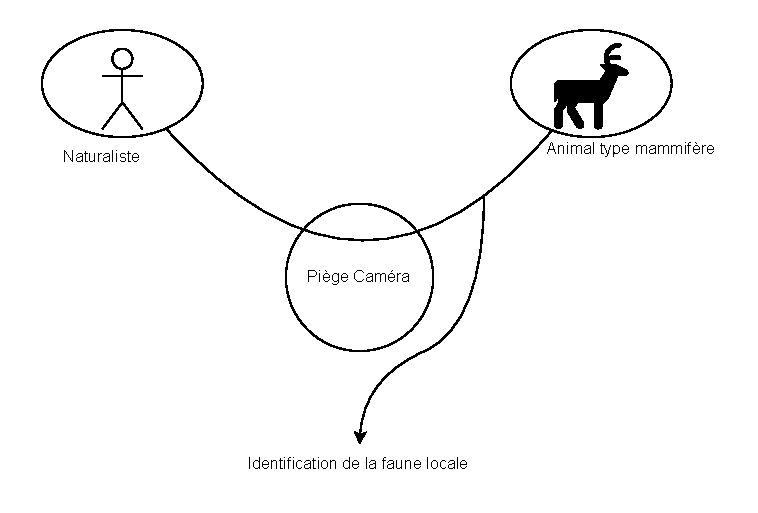
\includegraphics[width=0.7\textwidth]{images/bete_a_corne.pdf}
    }
    \caption{Bête à corne}
    \label{fig:BeteCor}
\end{figure}

\vspace{1cm}

\label{ann:DecFoncPrin}
\begin{figure}[h]
    \centering
    {
        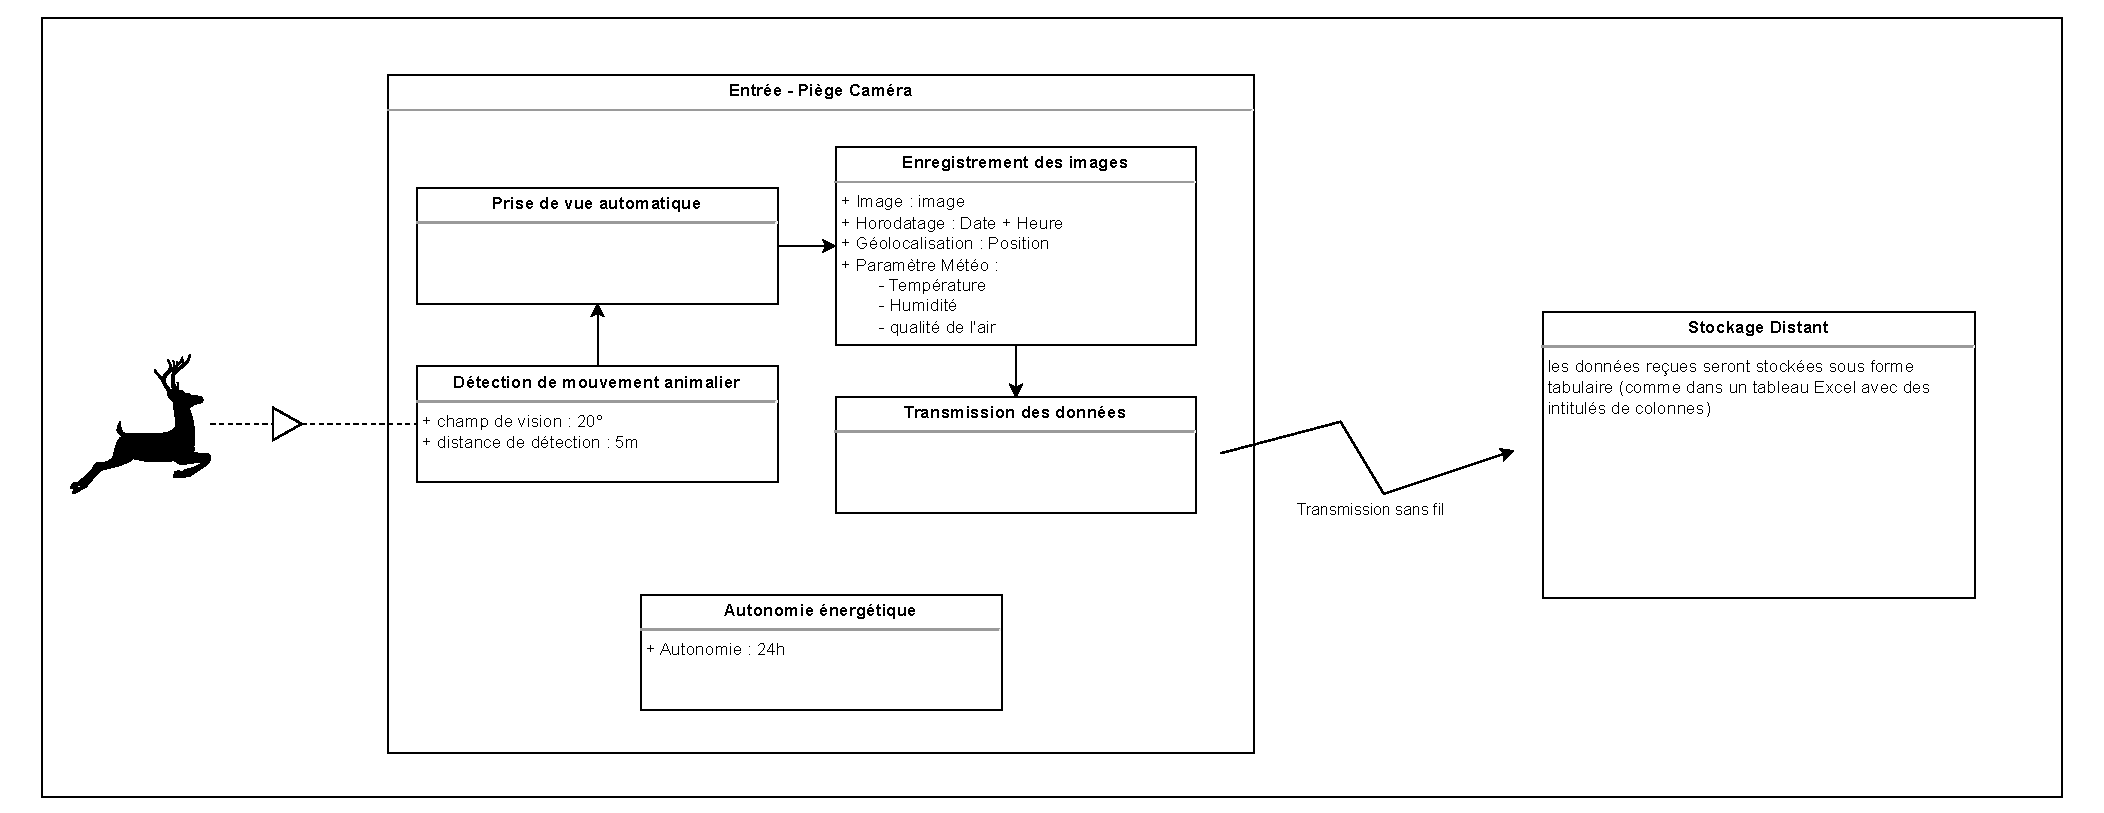
\includegraphics[width=1\textwidth]{images/schema_fonctionnel_principale.pdf}
    }
    \caption{Décomposition en bloc fonctionnel principale}
    \label{fig:DecFoncPrin}
\end{figure}

\label{ann:DecFoncGlo}
\begin{figure}[H]
    \centering
    {
        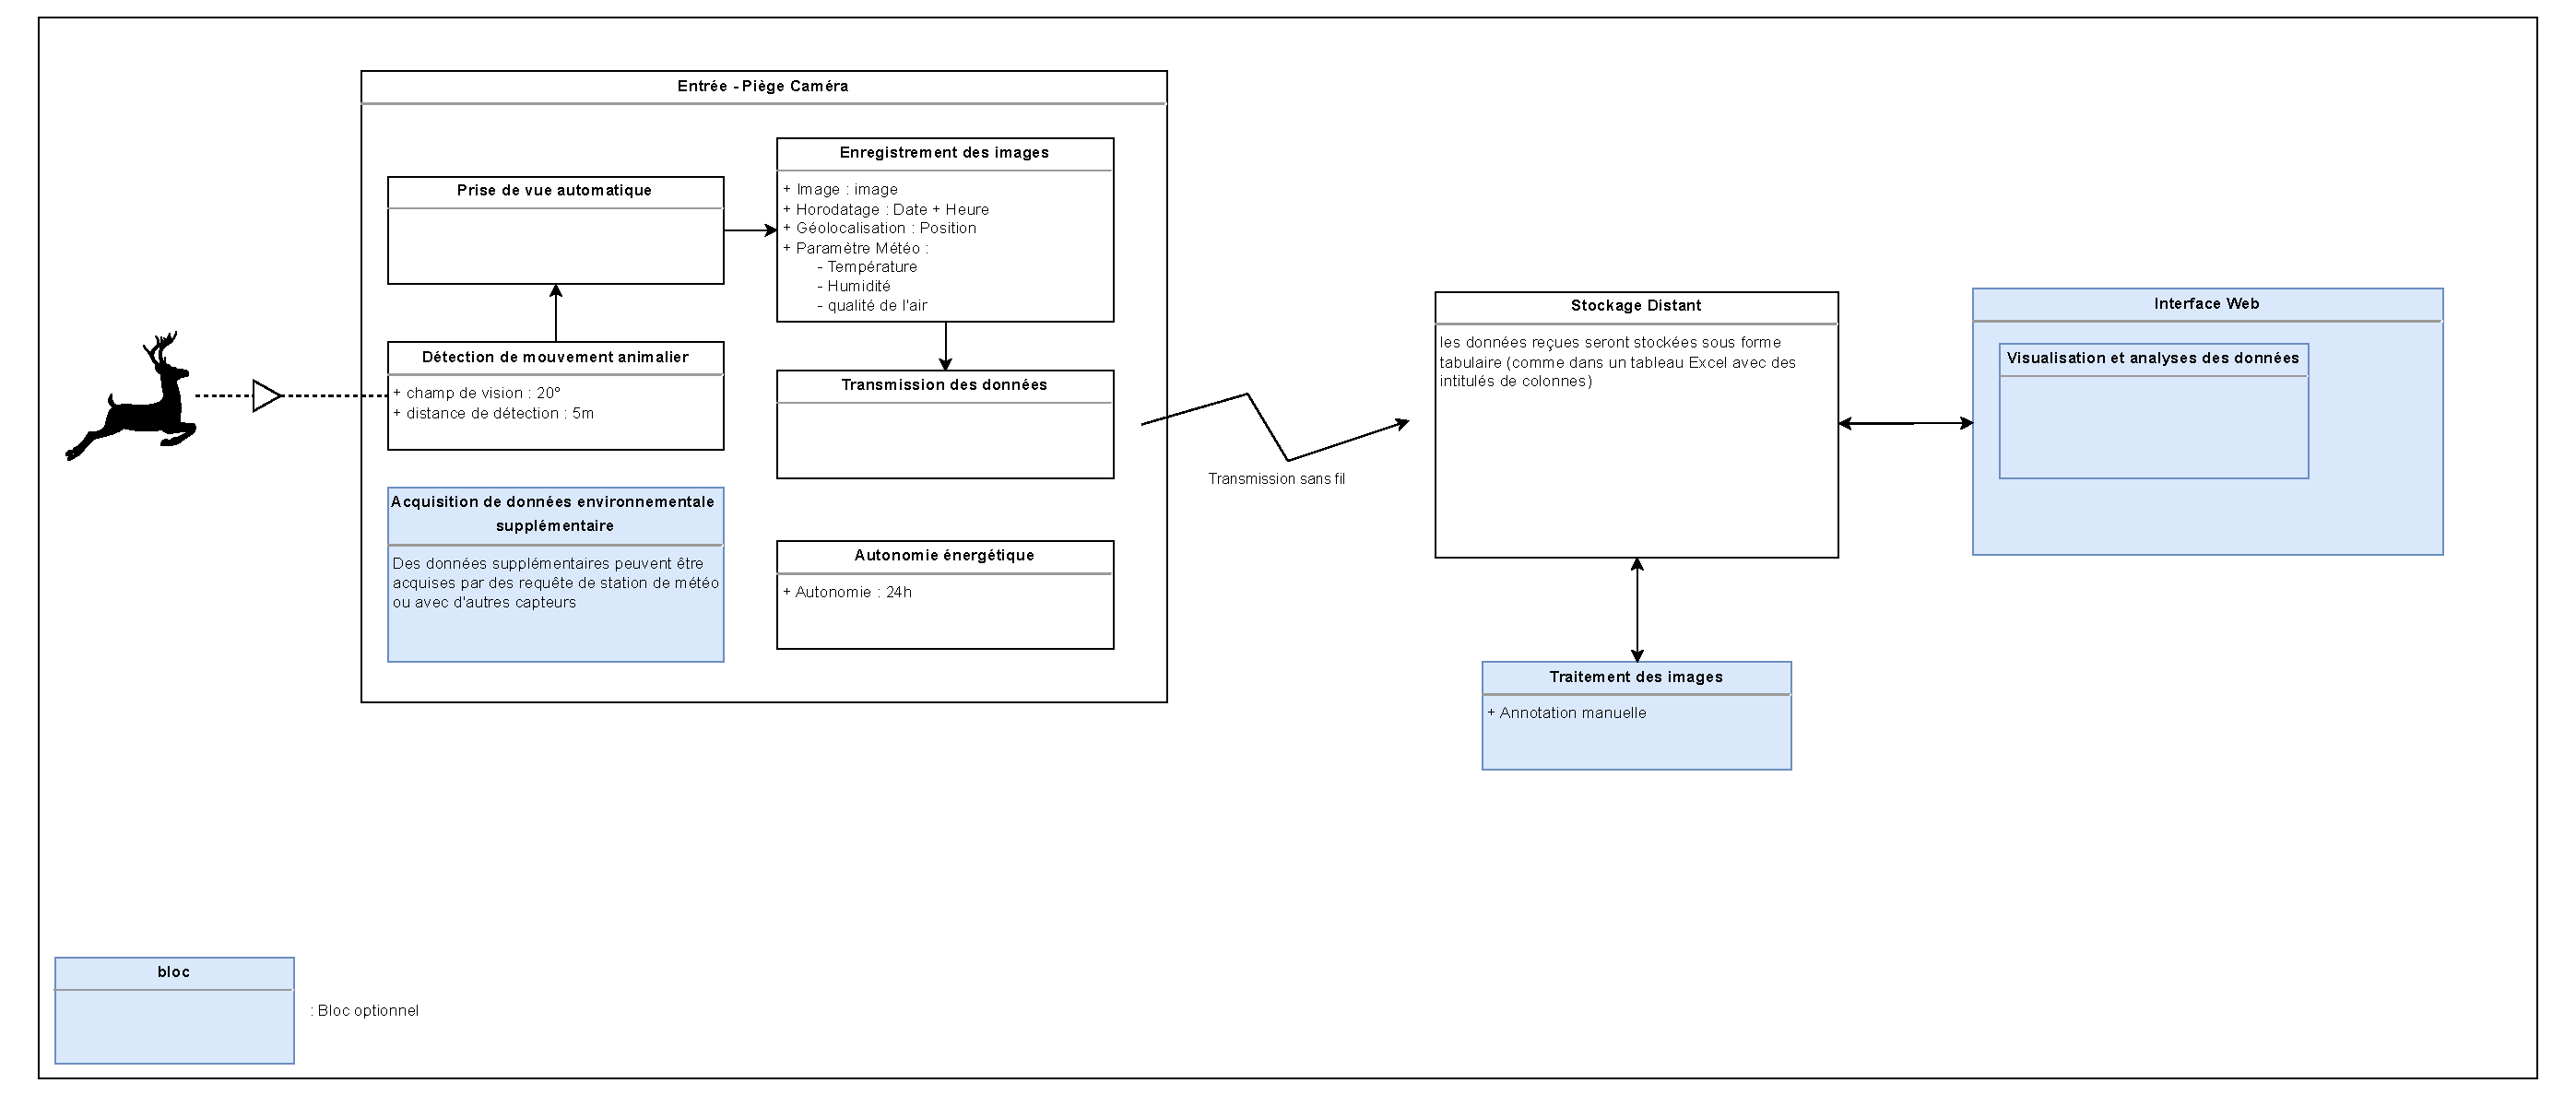
\includegraphics[width=1\textwidth]{images/schema_fontionnel_global.pdf}
    }
    \caption{Décomposition en bloc fonctionnel principale et optionnelle}
    \label{fig:DecFoncGlo}
\end{figure}

\vspace{1cm}

Afin de trouver la meilleur solution technique pour chaque work package du projet, un \gloss{benchmark} à été mis en place dans lequel les composants ou différentes solutions sont comparées selon différents critères. \\

\vspace{1cm}

% \begin{table}[h!]
%     \centering
%     \scriptsize
%     \begin{tabularx}{\textwidth}{|>{\raggedright\arraybackslash}p{2cm}|>{\raggedright\arraybackslash}p{2.2cm}|>{\raggedright\arraybackslash}p{1.8cm}|>{\raggedright\arraybackslash}p{1.5cm}|>{\raggedright\arraybackslash}p{2cm}|>{\raggedright\arraybackslash}p{2cm}|>{\raggedright\arraybackslash}p{1.5cm}|>{\raggedright\arraybackslash}p{1.8cm}|>{\centering\arraybackslash}p{0.8cm}|>{\centering\arraybackslash}p{1cm}|}
% \hline
%     \textbf{Mode} & \textbf{Principe} & \textbf{Portée typique} & \textbf{Débit indicatif} & \textbf{Avantages} & \textbf{Inconvénients} & \textbf{Coût / régulation} & \textbf{Cas d'usage} & \textbf{Énergie} & \textbf{Prix} \\
% \hline
%     Transmission HF \\ (modulation FM) & Radio HF (3–30 MHz) \\ modulation FM & Locale à mondiale \\ selon antenne & kb/s à \\ dizaines kb/s & Très grande portée, \\ robuste & Débit limité, \\ antennes \\ encombrantes & Autorisation \\ si > 5 W & Télécom longue \\ distance, backup & 5 W & 25 € \\
% \hline
%     LoRa & Modulation chirp \\ (LPWAN) & 0.5–15 km \\ selon environnement & 0.3 – 50 kb/s & Faible consommation, \\ grande portée & Débit limité, \\ duty-cycle & Faible coût, \\ pas d'abonnement & IoT capteurs, \\ télémétrie & 0,2 W & 30 € \\
% \hline
%     4G (LTE) & Réseau cellulaire & Couverture \\ nationale/ \\ internationale & 1–100+ Mb/s & Haut débit, \\ mobilité, \\ bonne latence & Payant (SIM), \\ énergivore & Abonnement, \\ licences & Vidéo, cloud, \\ gros volumes & 2 W & 70 € \\
% \hline
%     Réseau cartes \\ (filaire/sans fil) & SPI/I²C/RS485/ \\ BLE/Zigbee & $\sim$5–10 m \\ (selon solution) & Centaines kb/s \\ à plusieurs Mb/s & Simple, faible \\ latence, économique & Portée limitée, \\ dépend protocole & Faible coût & Robotique, \\ modules locaux & 0,1 W & Dépend \\ du µC \\
% \hline
%     Wi-Fi HaLow \\ (802.11ah) & Wi-Fi sub-GHz \\ pour IoT & Jusqu'à plusieurs \\ centaines de mètres & kb/s à \\ centaines kb/s & Longue portée \\ Wi-Fi, bonne \\ pénétration & Peu répandu, \\ matériel spécifique & Puces dédiées, \\ ISM & IoT longue portée, \\ réseaux capteurs & 0,7 W & 30 € \\
% \hline
%     ESP-NOW & Proto. Espressif \\ communication \\ directe Wi-Fi & 50–100 m (urbain), \\ 200–250 m (champ) & $\sim$1–2 Mb/s \\ (pratique <1 Mb/s) & Faible latence, \\ pas de routeur, \\ facile & Limité aux ESP, \\ pas de routage, \\ portée < LoRa & Très faible coût \\ (ESP32 < 5€) & Communication ESP \\ (robots, IoT local) & 1,5 W & 10 € \\
% \hline
%     \end{tabularx}
%     \caption{Comparatif des modes de transmission}
% \end{table}


\newgeometry{top=0cm, bottom=0cm, left=0cm, right=0cm}
\keepXColumns

\begin{landscape}
    \vspace*{\fill} % espace vertical avant le tableau

    \begin{table}[!ht]
        \centering % centre horizontalement
        \begin{tabularx}{\textwidth}{|p{2.5cm}|p{3cm}|p{3cm}|p{3cm}|p{2.5cm}|p{3cm}|p{3cm}|p{3.5cm}|p{1.5cm}|p{1.5cm}|}
            \hline
            \textbf{Mode}                     & \textbf{Principe}                              & \textbf{Portée typique}                & \textbf{Débit indicatif}           & \textbf{Avantages}                       & \textbf{Inconvénients}                          & \textbf{Coût / régulation}     & \textbf{Cas d'usage}                   & \textbf{Énergie} & \textbf{Prix} \\
            \hline
            Transmission HF (modulation FM)   & Radio HF (3–30 MHz) avec modulation FM         & Locale à mondiale selon antenne        & kb/s à dizaines kb/s               & Très grande portée, robuste              & Débit limité, antennes encombrantes             & Autorisation si > 5 W          & Télécom longue distance, backup        & 5 W              & 25 €          \\
            \hline
            LoRa                              & Modulation chirp  (LPWAN)                      & 0.5–15 km  selon environnement         & 0.3 – 50 kb/s                      & Faible consommation,  grande portée      & Débit limité,  duty-cycle                       & Faible coût,  pas d'abonnement & IoT capteurs,  télémétrie              & 0,2 W            & 30 €          \\
            \hline
            4G (LTE)                          & Réseau cellulaire                              & Couverture  nationale/  internationale & 1–100+ Mb/s                        & Haut débit,  mobilité,  bonne latence    & Payant (SIM),  énergivore                       & Abonnement,  licences          & Vidéo, cloud,  gros volumes            & 2 W              & 70 €          \\
            \hline
            Réseau cartes  (filaire/sans fil) & SPI/I²C/RS485/  BLE/Zigbee                     & $\sim$5–10 m  (selon solution)         & Centaines kb/s  à plusieurs Mb/s   & Simple, faible  latence, économique      & Portée limitée,  dépend protocole               & Faible coût                    & Robotique,  modules locaux             & 0,1 W            & Dépend  du µC \\
            \hline
            Wi-Fi HaLow  (802.11ah)           & Wi-Fi sub-GHz  pour IoT                        & Jusqu'à plusieurs  centaines de mètres & kb/s à  centaines kb/s             & Longue portée  Wi-Fi, bonne  pénétration & Peu répandu,  matériel spécifique               & Puces dédiées,  ISM            & IoT longue portée,  réseaux capteurs   & 0,7 W            & 30 €          \\
            \hline
            ESP-NOW                           & Proto. Espressif  communication  directe Wi-Fi & 50–100 m (urbain),  200–250 m (champ)  & $\sim$1–2 Mb/s  (pratique <1 Mb/s) & Faible latence,  pas de routeur,  facile & Limité aux ESP,  pas de routage,  portée < LoRa & Très faible coût  (ESP32 < 5€) & Communication ESP  (robots, IoT local) & 1,5 W            & 10 €          \\
            \hline
        \end{tabularx}
        \caption{Comparaison des différentes technologies de transmission possible} % légende après le tableau
        \addcontentsline{lof}{figure}{\thetable\quad \hspace{6pt}Comparaison des différentes technologies de transmission possible}
    \end{table}

    \vspace*{\fill} % espace vertical après le tableau

    \begin{table}[!ht]
        \centering
        \begin{tabularx}{\textwidth}{
            |p{3cm}|p{2.5cm}|p{2.5cm}|p{2cm}|
            p{2.5cm}|p{3cm}|p{3cm}|p{1.5cm}|p{2cm}|p{2cm}|
            }
            \hline
            \textbf{Caméra}               & \textbf{Capteur}         & \textbf{Résolution max}   & \textbf{Interface} &
            \textbf{Format vidéo / image} & \textbf{Points forts}    & \textbf{Points faibles}   &
            \textbf{Prix indicatif}       & \textbf{Champ de vision} & \textbf{Énergie (active)}                                                                                                                                                                             \\
            \hline
            OV7670                        & CMOS VGA                 & 640×480                   & Parallèle / SCCB   & YUV / RGB           & Très bon marché, faible consommation                     & Résolution faible                            & 5 €  & 25°  & 0,06 W \\
            \hline
            OV2640                        & CMOS                     & 1600×1200                 & SCCB / parallèle   & JPEG / RGB          & JPEG intégré, bonne résolution                           & Débit limité                                 & 15 € & 160° & 0,14 W \\
            \hline
            Raspberry Pi Camera V2        & Sony IMX219              & 8 MP                      & CSI-2              & MJPEG / H.264 / RAW & Haute qualité vidéo, compatible Pi                       & Nécessite Pi                                 & 17 € & 62°  & 0,3 W  \\
            \hline
            ESP32-CAM                     & OV2640                   & 1600×1200                 & Wi-Fi / GPIO       & JPEG / MJPEG        & Caméra + Wi-Fi intégré, compact                          & Streaming HD limité                          & 13 € & 160° & 0,14 W \\
            \hline
            Raspberry Pi HQ Camera        & Sony IMX477R             & 12.3 MP                   & CSI-2              & RAW12/10/8, COMP8   & Très haute qualité, objectifs interchangeables           & Nécessite Pi, coûteux                        & 58 € & 75°  & 0,3 W  \\
            \hline
            Arducam 5MP / 8MP Mini Module & OV5640 / OV5647          & 5–8 MP                    & SPI / I²C          & JPEG / RAW          & Compact, résolution suffisante, compatible Arduino / ESP & Configuration parfois complexe, nécessite Pi & 30 € & --   & 0,4 W  \\
            \hline
            Pi NoIR Camera V2             & Sony IMX219 (NoIR)       & 8 MP                      & CSI-2              & MJPEG / H.264 / RAW & Vision nocturne IR, compatible Pi                        & Nécessite Pi                                 & 30 € & --   & 0,3 W  \\
            \hline
            Arducam IMX219 NoIR           & Sony IMX219 (NoIR)       & 8 MP                      & SPI / I²C / CSI    & JPEG / RAW          & Vision nocturne, module compatible Pi / Arduino          & Plus cher que OV2640, nécessite Pi           & 40 € & --   & 0,3 W  \\
            \hline
        \end{tabularx}
        \caption{Comparaison des modules caméras}
        \addcontentsline{lof}{figure}{\thetable\quad \hspace{6pt}Comparaison des modules caméras}
    \end{table}

    \begin{table}[!ht]
        \centering
        \begin{tabularx}{\textwidth}{
            |p{3.5cm}|p{2.5cm}|p{2.2cm}|p{1.2cm}|p{1.4cm}|
            p{2.7cm}|p{2.5cm}|p{3cm}|p{3cm}|p{1.8cm}|p{2.2cm}|
            }
            \hline
            \textbf{Microcontrôleur / Carte} & \textbf{Processeur} & \textbf{Fréquence}    & \textbf{RAM}            & \textbf{Flash} &
            \textbf{Connectivité}            & \textbf{GPIO / I/O} & \textbf{Points forts} & \textbf{Points faibles} &
            \textbf{Prix indicatif}          & \textbf{Puissance}                                                                                                                                                                                                                                 \\
            \hline
            Arduino Uno (ATmega328P)         & AVR 8-bit           & 16 MHz                & 2 KB                    & 32 KB          & USB / UART             & 14 digital / 6 analog  & Très simple, stable, énorme support communauté & Faible puissance, mémoire limitée   & 20 €   & 0.30 W  \\
            \hline
            Arduino Nano 33 BLE              & ARM Cortex-M4       & 64 MHz                & 32 KB                   & 256 KB         & BLE                    & 14 digital / 8 analog  & BLE intégré, faible consommation, compact      & Plus cher que Nano classique        & 22.5 € & 0.035 W \\
            \hline
            Arduino Mega 2560                & AVR 8-bit           & 16 MHz                & 8 KB                    & 256 KB         & USB / UART             & 54 digital / 16 analog & Beaucoup de GPIO, support shield               & Lent, mémoire RAM limitée           & 25 €   & 0.357 W \\
            \hline
            SAMD21                           & ARM Cortex-M0+      & 48 MHz                & 32 KB                   & 256 KB         & USB / UART             & 14 digital / 6 analog  & Faible consommation, 32-bit                    & Moins répandu que Uno               & 20 €   & 0.025 W \\
            \hline
            STM32F103C8 (Blue Pill)          & ARM Cortex-M3       & 72 MHz                & 20 KB                   & 64 KB          & USB / UART / SPI / I²C & 37 digital / 10 analog & Puissant, rapide, compact, pas cher            & Écosystème moins simple que Arduino & 5 €    & 0.01 W  \\
            \hline
        \end{tabularx}
        \caption{Comparaison des microcontrôleurs}
        \addcontentsline{lof}{figure}{\thetable\quad \hspace{6pt}Comparaison des microcontrôleurs}
    \end{table}

    \begin{table}[!ht]
        \centering
        \begin{tabularx}{\textwidth}{
            |p{3.5cm}|p{2.5cm}|p{2.2cm}|p{1.2cm}|p{1.4cm}|
            p{2.7cm}|p{2.5cm}|p{3cm}|p{3cm}|p{1.8cm}|p{2.2cm}|
            }
            \hline
            \textbf{Microcontrôleur / Carte} & \textbf{Processeur}               & \textbf{Fréquence}    & \textbf{RAM}            & \textbf{Flash} &
            \textbf{Connectivité}            & \textbf{GPIO / I/O}               & \textbf{Points forts} & \textbf{Points faibles} &
            \textbf{Prix indicatif}          & \textbf{Puissance}                                                                                                                                                                                                                                                                                     \\
            \hline
            ESP8266                          & Tensilica 32-bit                  & 80–160 MHz            & 160 KB                  & 4 MB           & Wi-Fi                & 17 digital / 1 analog  & Wi-Fi intégré, petit, bon marché                                       & Moins de GPIO, pas BLE                              & 4 €    & 0.4 W   \\
            \hline
            ESP32                            & Tensilica Xtensa dual-core 32-bit & 240 MHz               & 520 KB                  & 4 MB           & Wi-Fi + BLE          & 34 digital / 18 analog & Wi-Fi + BLE intégré, puissant                                          & Plus complexe à programmer que Arduino classique    & 8 €    & 0.7 W   \\
            \hline
            ESP32-CAM                        & Tensilica Xtensa 32-bit           & 240 MHz               & 520 KB                  & 4 MB           & Wi-Fi + BLE          & Caméra + GPIO          & Caméra + Wi-Fi intégré, compact                                        & Pas facile pour debugging, consommation plus élevée & 9.5 €  & 1.25 W  \\
            \hline
            Raspberry Pi 4                   & ARM Cortex-A72 quad-core          & 1.5 GHz               & 2–8 GB                  & SD Card        & Ethernet, Wi-Fi, BLE & GPIO 40 broches        & Puissant, Linux, multi-tâches, HDMI, USB                               & Consommation élevée, pas microcontrôleur pur        & 55 €   & 4 W     \\
            \hline
            Raspberry Pi Zero                & ARM1176JZF-S                      & 1 GHz                 & 512 MB                  & SD Card        & Wi-Fi / BLE (Zero W) & GPIO 40 broches        & Petit, faible coût, Linux                                              & Faible puissance CPU, Linux obligatoire             & 12.5 € & 0.7 W   \\
            \hline
            Raspberry Pi Pico                & RP2040 dual-core ARM Cortex-M0+   & 133 MHz               & 264 KB                  & 2 MB           & USB                  & 26 digital / 3 analog  & Très bon compromis prix/puissance, RP2040 programmable C / MicroPython & Pas de Wi-Fi natif                                  & 5 €    & 0.135 W \\
            \hline
        \end{tabularx}
        \caption{Comparaison des microcontrôleurs (suite)}
        \addcontentsline{lof}{figure}{\thetable\quad \hspace{6pt}Comparaison des microcontrôleurs (suite)}
    \end{table}

    % \begin{table}[!ht]
    % \centering
    % \small
    % \begin{tabularx}{\textwidth}{
    % |p{2.5cm}|p{2cm}|p{2cm}|p{2cm}|p{2cm}|
    % p{2.5cm}|p{1.8cm}|p{1.5cm}|p{1.8cm}|p{1.8cm}|
    % p{2.8cm}|p{2.8cm}|p{3cm}|p{2.8cm}|p{2cm}|
    % }
    % \hline
    % \textbf{Nom du capteur} & \textbf{Module} & \textbf{Type} & \textbf{Tension} & \textbf{Interface} & 
    % \textbf{Plateforme principale} & \textbf{Courant typique} & \textbf{Puissance} &
    % \textbf{Prix (Amazon)} & \textbf{Prix (AliExpress)} &
    % \textbf{Avantages} & \textbf{Inconvénients} & 
    % \textbf{Description / Application} & \textbf{Lien fiche technique} & \textbf{Remarques} \\
    % \hline
    % HC-SR501 PIR & Détection de mouvement & Capteur infrarouge passif & 4.5–12 V & GPIO & ESP32 / STM32 / Arduino & 65 µA & 0,0003 W & 5.50 € & 1.95 € & Faible consommation, coût réduit & Peu sensible aux mouvements lents ou aux fortes températures & Détection du rayonnement thermique pour déclencher photo ESP32-CAM & components101.com/sensors/hc-sr501-pir-sensor & Solution principale \\
    % \hline
    % AM312 Mini PIR & Détection de mouvement & Mini-capteur infrarouge & 2.7–12 V & GPIO & ESP32 / Arduino & 15 µA & 0,00004 W & 3.90 € & 1.40 € & Très basse consommation, taille compacte & Portée courte, sensibilité non réglable & Adapté aux systèmes solaires & alldatasheet.com/AM312 & Option \\
    % \hline
    % RCWL-0516 & Détection de mouvement & Radar micro-ondes Doppler & 4–28 V & GPIO & ESP32 / Raspberry Pi & 2.8 mA & 0,0112 W & 7.40 € & 1.45 € & Traverse le plastique/verre/bois, insensible T°, très réactif & Sensible aux interférences RF, portée variable & Détection de mouvement par effet Doppler & handsontec.com/dataspecs/sensor/radar-sensor.pdf & Non essentiel \\
    % \hline
    % HC-SR04 & Détection de mouvement & Capteur ultrasonique & 5 V & GPIO (Trig/Echo) & Arduino / STM32 & 15 mA & 0,075 W & 4.20 € & 1.05 € & Mesure précise (2 cm–4 m), insensible à la lumière & Sensible à T°, vent, surfaces molles & Mesure de distance / obstacles & sparkfun.com/datasheets/Sensors/Proximity/HCSR04.pdf & Option \\
    % \hline
    % MLX90640 & Détection de mouvement & Matrice IR thermique (32×24) & 3.0–3.6 V & I²C & ESP32 / RPi / Arduino & 23 mA & 0,069 W & 52.50 € & 29.50 € & Image thermique temps réel, haute précision & Coût élevé, traitement image requis & Cartographie thermique d’animaux ou humains & melexis.com/datasheet-mlx90640 & Non essentiel \\
    % \hline
    % \end{tabularx}
    % \caption{Comparaison des capteurs afin des récupérer les méthadonnées lié aux photos}
    % \end{table}

    % \begin{table}[!ht]
    % \centering
    % \small
    % \begin{tabularx}{\textwidth}{
    % |p{2.5cm}|p{2.5cm}|p{2.8cm}|p{2cm}|p{2cm}|
    % p{2.5cm}|p{1.8cm}|p{1.5cm}|p{1.8cm}|p{1.8cm}|
    % p{2.8cm}|p{2.8cm}|p{3cm}|p{2.8cm}|p{2cm}|
    % }
    % \hline
    % \textbf{Nom du capteur} & \textbf{Module} & \textbf{Type} & \textbf{Tension} & \textbf{Interface} &
    % \textbf{Plateforme principale} & \textbf{Courant typique} & \textbf{Puissance} &
    % \textbf{Prix (Amazon)} & \textbf{Prix (AliExpress)} &
    % \textbf{Avantages} & \textbf{Inconvénients} &
    % \textbf{Description / Application} & \textbf{Lien fiche technique} & \textbf{Remarques} \\
    % \hline
    % DHT22 & Surveillance environnementale & Température / humidité & 3.5–5.5 V & 1-Wire & Toutes plateformes & 2.5 mA & 0,00875 W & 9.50 € & 1.45 € & Bonne précision, facile d’usage & Réponse lente (~2 s), non étanche & Mesure T° et humidité & components101.com/sensors/dht22 & Option \\
    % \hline
    % BME280 & Surveillance environnementale & Température / humidité / pression & 1.71–3.6 V & I²C / SPI & ESP32 / RPi & 0.6 mA & 0,00216 W & 8.50 € & 3.00 € & Haute précision, faible conso, 3-en-1 & Non étanche, plus cher & Capteur principal T°/RH/Pression & bosch-sensortec.com/bst-bme280 & Solution principale \\
    % \hline
    % BME680 & Surveillance environnementale & T°, RH, pression + qualité d’air & 1.71–3.6 V & I²C / SPI & ESP32 / RPi & 2–3 mA & 0,0108 W & 17.00 € & 5.00 € & Mesure 4 paramètres, haute stabilité & Coût élevé, chauffe nécessaire & Capteur avancé qualité d’air & octopart.com/datasheet/bme680 & Extension \\
    % \hline
    % BH1750 & Surveillance environnementale & Luminosité (lux) & 2.4–3.6 V & I²C & Toutes plateformes & 0.12 mA & 0,000432 W & 6.00 € & 3.00 € & Haute sensibilité, insensible IR & Ne mesure pas IR/UV, inutilisable dans le noir & Mesure lumière ambiante & components101.com/sensors/bh1750 & Non essentiel \\
    % \hline
    % Rain Sensor & Surveillance environnementale & Détection de pluie & 5 V & A0 + D0 & Arduino / STM32 & 3–15 mA & 0,075 W & 4.00 € & 1.50 € & Sensibilité réglable, sortie analog+numérique & Non étanche, sensible à la poussière & Détection humidité de surface & components101.com/sensors/rain-drop-sensor-module & Non essentiel \\
    % \hline
    % \end{tabularx}
    % \caption{Comparaison des capteurs afin des récupérer les méthadonnées lié aux photos (suite - 1)}
    % \end{table}

    % \begin{table}[!ht]
    % \centering
    % \small
    % \begin{tabularx}{\textwidth}{
    % |p{2.5cm}|p{2.5cm}|p{2.8cm}|p{2cm}|p{2cm}|
    % p{2.5cm}|p{1.8cm}|p{1.5cm}|p{1.8cm}|p{1.8cm}|
    % p{2.8cm}|p{2.8cm}|p{3cm}|p{2.8cm}|p{2cm}|
    % }
    % \hline
    % \textbf{Nom du capteur} & \textbf{Module} & \textbf{Type} & \textbf{Tension} & \textbf{Interface} &
    % \textbf{Plateforme principale} & \textbf{Courant typique} & \textbf{Puissance} &
    % \textbf{Prix (Amazon)} & \textbf{Prix (AliExpress)} &
    % \textbf{Avantages} & \textbf{Inconvénients} &
    % \textbf{Description / Application} & \textbf{Lien fiche technique} & \textbf{Remarques} \\
    % \hline
    % MAX9814 & Audio & Micro analogique (AGC) & 2.7–5.5 V & Analog / I²S & ESP32 / STM32 & 3 mA & 0,0165 W & 7.00 € & 1.45 € & AGC intégré, faible bruit & Sensible aux bruits ambiants & Détection des sons d’animaux ou environnementaux & analog.com/MAX9814.pdf & Solution principale \\
    % \hline
    % SPH0645LM4H-B & Audio & Micro numérique MEMS & 1.62–3.6 V & I²S & ESP32 / RPi & 0.6 mA & 0,00216 W & 4.50 € & 2.50 € & Sortie numérique stable, très faible conso & Pas de sortie analogique & Capture audio numérique I²S & digikey.fr/SPH0645LM4H-B & Option \\
    % \hline
    % NEO-6M GPS & Localisation / GPS & Récepteur satellite & 3.0–5.0 V & UART & ESP32 / Arduino / RPi & 35 mA & 0,175 W & 10.00 € & 8.50 € & Haute précision, faible coût & Nécessite ciel dégagé & Donne la position GPS et l’heure UTC & octopart.com/datasheet/neo-6m-0-001-u-blox & Option \\
    % \hline
    % SIM7600E-H & Localisation / GPS & Module 4G + GNSS & 3.4–4.2 V & UART / USB / GNSS & ESP32 / STM32 / RPi & 200–500 mA (TX crête) & 2,1 W & 70.00 € & 40.00 € & Communication 4G LTE + GPS & Prix et conso élevés & Envoi d’images / SMS 4G + localisation & simcom/SIM7600E-H.pdf & Option \\
    % \hline
    % MPU-6050 & Orientation / Mouvement & Accéléromètre + gyroscope & 2.375–3.46 V & I²C & Toutes plateformes & 3.9 mA & 0,0135 W & 5.00 € & 2.00 € & Compact, bon rapport qualité/prix & Précision limitée & Détection d’inclinaison et vibrations & invensense MPU-6050 & Solution principale \\
    % \hline
    % MPU-9250 & Orientation / Mouvement & Accéléro + gyro + magnétomètre & 2.4–3.6 V & I²C / SPI & ESP32 / RPi & 3.7 mA & 0,0133 W & 11.50 € & 2.00 € & Capteur 9 axes, haute sensibilité & Prix plus élevé & Suivi de mouvement et orientation & alldatasheet.com/MPU-9250 & Option \\
    % \hline
    % INA219 & Surveillance énergétique & Capteur de courant / tension & 3.0–5.5 V & I²C / SMBus & Toutes plateformes & 1 mA & 0,0055 W & 7.00 € & 2.00 € & Haute précision, mesure bidirectionnelle & Plage limitée & Suivi tension et puissance batterie & ti.com/INA219 & Extension \\
    % \hline
    % \end{tabularx}
    % \caption{Comparaison des capteurs afin des récupérer les méthadonnées lié aux photos (suite - 2)}
    % \end{table}

\end{landscape}
